\chapter{Design}

With the features discussed in \autoref{sec:KubeLB}, the next step is to think about how we could achieve the needed features.
Since the core product of Kubermatic is based on Kubernetes, the KubeLB project is also to be operated in this context.
To use concepts from KKP, the goal is to use a Kubernetes cluster for load balancing.
This promotes a homogeneous environment of Kubernetes clusters without introducing additional complexity of third party systems, which simplifies both the deployment and the maintenance of the KubeLb application.

\section{Manager}

The Manager, will serve as an operator, as already explained in \autoref{sec:operator-pattern} and implement a controller like in \autoref{sec:controllers}.
Its task is to take care of the configuration of the load balancer within the load balancer cluster.

Within the load balancing cluster, different Kubernetes resources are used for this purpose.
\\
The deployment \autoref{subsec:deployment} creates the actual load balancer within the cluster.
\\
The service \autoref{subsec:service} exposes the load balancer deployment to the outside via a service type LoadBalancer.
It should be noted that the LB cluster requires a load balancer implementation.
This can be either a cloud provider, or an opensource single cluster implementation.
\\
Since the created service is of type load balancer, the status field of the service gets updated with the external IP address.
The manager recognizes this and sets the status field within the CRD.
\\
For layer 7 implementation, the Manager makes use of the Ingress\autoref{subsec:ingress}, therefore any Ingress Controller \autoref{sec:IngressController} musst be installed as well.

\section{Agent}

The Agent runs inside a User Cluster and watch for Services and Ingress Resources.
If needed it creates a CRD with the details needed for the Manager to do the load balancing.
Since the agent runs inside the user cluster, it can read the desired configurations of the service or ingress resource and create, modify or delete the CRD appropriately.
\\
Likewise, it is able to get the endpoints and open ports for the service for LoadBalancing.
Since the cluster size, i.e.\ the number of nodes, can change dynamically, it is also the agent's task to update the changed endpoints of the user cluster for all CRD's within the LB cluster.
\\
In the case of Layer 4 load balancing, the Agent also sets the IP address in the status field of the service, which is set inside the status field of the CRD by the Manger.
\\
To interact with the LB cluster, the agent needs access to a namespace for the CRDs.

\section{Layer 4}

\autoref{fig:kubelb-l4} illustrates the architecture of Layer 4 load balancing.
Within the user cluster, the agent observes the service resource.
If a user creates a service of type LoadBalancer, the Agent recognizes the service and creates a TCPLoadBalancer inside the LB Cluster.
\\
The manager observes the TCPLoadBalancer CRD, which contains the necessary information to configure the load balancer.
Based on this, the manager creates or updates the load balancer deployment and the associated service.


\begin{figure}[H]
    \centering
    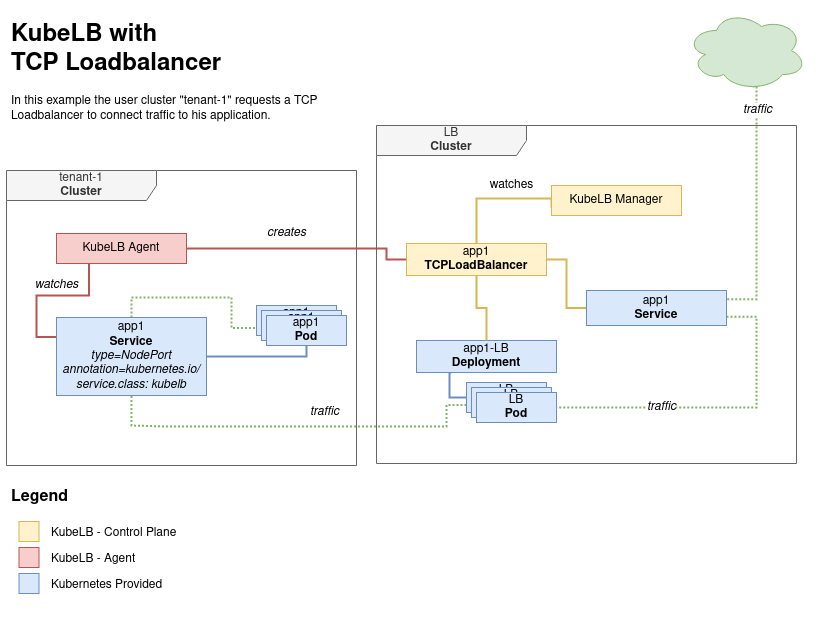
\includegraphics[width=1\linewidth]{media/06/kubelb-l4}
    \caption{"KubeLB Layer 4 architecture"  by Kubermatic GmbH Apache License 2.0}
    \label{fig:kubelb-l4}
\end{figure}

\section{Layer 7}

Layer 7 load balancing has a bit more complexity, as \autoref{fig:kubelb-l7} shows, it relies on more components.

In normal Kubernetes the IngressController serve as an entrypoint, because we don't have an ingressController installed inside the user cluster some extra steps are required.
At first the Service to expose via Ingress is probably of type ClusterIp, therefore it is not reachable for the load balancer inside the LB Cluster.
In this case the Agent copies the existing service and creates a new one of type node port, so it is actually exposed and accessible to the load balancer.
\\
The second part is to create a TCPLoadBalancer, based on the copied service, inside the LB Cluster.
Since KubeLb makes use of the IngressController implementation, it needs some Kind of Connector to the outside of the Cluster.
Ingress is by design cluster based and only routable to internal services, so for that reason its mandatory to have a LoadBalancer service inside the LB Cluster.
It is not necessary to expose the load balancer, so the agent sets the service type inside the TCPLoadBalancer to Clusterip.
\\
At this point the Agent creates a HTTPLoadBalancer, based on the Ingress inside the User cluster, inside the LB Cluster.
The Manager takes care that the Ingress is configured to use the corresponding LoadBalancer service, which was created before.


\begin{figure}[H]
    \centering
    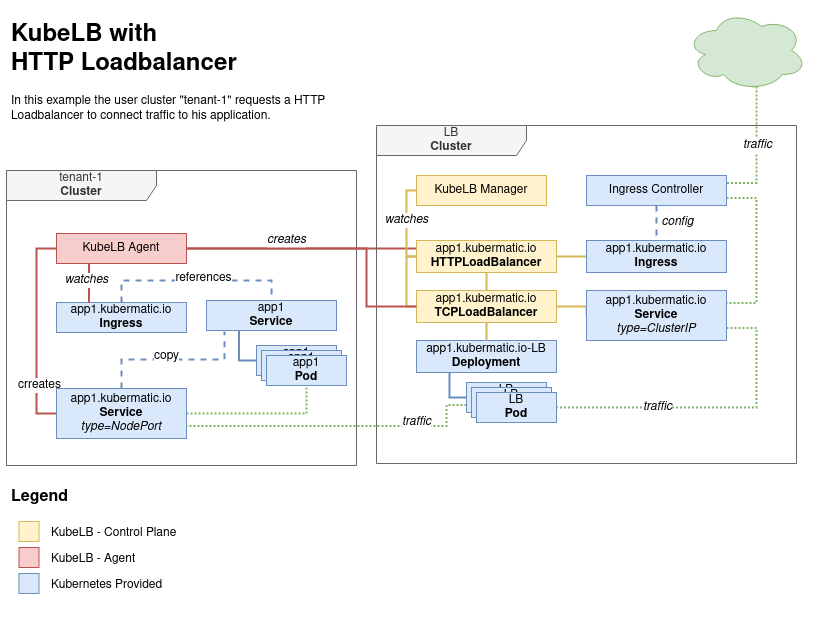
\includegraphics[width=1\linewidth]{media/06/kubelb-l7}
    \caption{"KubeLB Layer 7 architecture"  by Kubermatic GmbH Apache License 2.0}
    \label{fig:kubelb-l7}
\end{figure}

\section{Envoy}

Envoy will serve as a load balancer instance due to its design for large modern service oriented architectures and high level feature set
\\
The following describes the most important functions needed for KubeLB.

\begin{itemize}
    \item \textit{L3/L4 filter architecture} \\
    The envoy core is a L3/L4 network proxy, that is configurable via filter chains, allowing the proxy to perform different TCP/UDP tasks.
    \item \textit{HTTP L7 filter architecture} \\
    Since HTTP is widely used for applications to communicate, envoy offers an additional Layer 7 filter architecture on top, which can be used for various tasks like rate limiting, routing, forwarding and more.
    \item \textit{HTTP L7 routing} \\
    Envoy offers a special Layer 7 routing filter to make HTTP header based routing decisions and more.
    \item \textit{Advanced load balancing} \\
    It implements a rich set of load balancing algorithms, as well as automatic retries, circuit breaking.
    \item \textit{Health checking} \\
    Envoy supports active and also passive health checking, to determine healthy endpoint targets.
\end{itemize}

This is just a brief overview of what KubeLB is probably going to make use of.~\cite{WHAT-IS-ENVOY}
\\
Another important feature is its data plane api.
In contrast to a control-plane the data-plane controls the data requests.
\\
To fulfill that purpose the Envoy api implements a data-plane.
In Practice that means it is possible to control envoy proxies via this api.
This is very useful in cloud native environments, where services change their configuration on runtime, nodes get added or deleted and so on.
For that reason the Manager can implement the envoy data-plane api and control the current configuration of all it's load balancers.
